% input files
\begin{center}
    % \LARGE \textsc{Заметки по практике \\ <<Квантовые вычисления на холодных атомах и ионах>>}
    % \Large \textsc{Задания по практике
    %  <<Квантовая механика>>
    \Large \textsc{Семинары по Статистической Фиpике}
\end{center}

\hrule

\phantom{42}

\begin{flushright}
    \begin{tabular}{rr}
    % written by:
    \textbf{Семинарист}:
    	& Белемук А.М. \\
        \textbf{Автор}:  
        & Примак Евгений\\
    \end{tabular}
\end{flushright}

\begin{figure}[h]
    \centering
    \includegraphics[width=0.7\textwidth]{img/St_John_the_Baptist_in_the_Wilderness.jpg}
    %\caption{}
    %\label{fig:}
\end{figure}

\newpage

\thispagestyle{empty}
\tableofcontents
\newpage

\setcounter{section}{1}
\section{Cеминар}
\subsubsection*{Адиабатическое размагничивание (задача)}
Имеем кристаллическую решетку с примесями. (Магнито-каллорический эффект)
\begin{equation*}
	E = E_{\text{поле решетки}} + E_{\text{примесей в малом поле}},
\end{equation*}
если $H$ -- понижаем, то $T$ образца уменьшается. Нужно найти $\frac{\partial T}{\partial H} - ?$.

\subsubsection*{Будем решать.}

Функцией чего является энергия? $E(S,V H)$. Пренебрегаем изменением $V$, то есть объём фиксирован.
\begin{equation*}
	d E = T d S - M d H
\end{equation*}
тогда
\begin{equation*}
	\left(\frac{\partial T}{\partial H}\right)_{S} = - \left(\frac{\partial M}{\partial S}\right)_{H} 
	= - \frac{\partial (M, H)}{\partial (T, H)}
	= - \frac{\partial(M, H)}{\partial(T,H)} \frac{\partial(T, H)}{\partial(S,H)}
	= - \left(\frac{\partial M}{\partial T}\right)_H \cdot \frac{T}{T (\partial S/\partial T)_H} 
	= \left(- \frac{\partial M}{\partial T}\right)_H \frac{T}{C_{V, H}}
\end{equation*}
Кроме того теплоёмкость системы, примесная же теплоёмкость это
\begin{equation*}
	C = C_\text{решетки} + C_\text{примесей} \approx C_{V, H} \approx \alpha T^3.
\end{equation*}
Парамагнетик в слабых полях (закон Кюри): 
$$M(T) = \chi(T) H, \hspace{1 cm}\chi(T) = A/T.$$ Таким образом
\begin{equation*}
	\left(\frac{\partial M}{\partial T}\right)_H = \chi'(T) H;
	\hspace{1 cm}
	\left(- \frac{\partial M}{ \partial T}\right)_H = \frac{A}{T^2} H
\end{equation*}
Таким образом 
\begin{equation*}
	\left(\frac{\partial T}{ \partial H}\right)_S = \frac{A}{T^2} H \frac{T}{\alpha T^3} = \frac{A H}{\alpha T^4}.
\end{equation*}
Следовательно, 

Если $H$ увеличиваем, то $ T$ --- увеличивается. Если $H$ уменьшается, то $T$ --- уменьшается.

\subsubsection*{Двухуровневая Система}
Имеем $N$ атомов, часть из них $n$ на возбужденном уровне. Тогда задана и энергия системы
\begin{equation*}
	E_{\text{сист}} = 0 \cdot (N - n) + n \varepsilon = n \varepsilon.
\end{equation*}
Наша задача найти $S(E) - ?$ (и всё так далее про термодинамику)

И так, задание $(N, n)$ однозначно определяет $(N, E)$ и наоборот. Энтропия будет функцией $S(E,N)$.
И по Больцману 
\begin{equation*}
	S = \ln W(E),
\end{equation*}
где $W(E)$ -- статистический вес -- число микроскопических состояний, отвечающих заданному макросостоянию.
Число таких микросотояний легко посчитать $W(E) = C_N^n = \frac{N!}{n! (N-n)!}$.

По формуле Стирлинга
\begin{equation*}
	N! \approx \left(\frac{N}{e}\right)^{N}, 
	\hspace{1 cm}
	\ln N! \approx N \ln N - N.
\end{equation*}
Тогда
\begin{align*}
	\ln C_N^n &\approx \ln N! - \ln n! = \ln(N-n)! = N\ln N - N - n \ln n + n - (N-n) \ln(N-n) + N - n \\
	&= N \ln N - n \ln n - (N-n) \ln N - (N-n) \ln\left(1- \frac{n}{N}\right) \\
	& = - n \ln\frac{n}{N} - N \left(1 - \frac{n}{N}\right) \ln\left(1 - \frac{n}{N}\right) \\
	& = N \left[- \frac{n}{N} \ln \frac{n}{N} - \left(1 - \frac{n}{N}\right) \ln \left(1 - \frac{n}{N}\right)\right] = S
\end{align*}
Энтропия у нас пропорциональная $N$, а в скобках там стоит плотность $n/N = x$ -- доля возбужденных атомов.
\begin{equation*}
	E = \varepsilon n 
	\hspace{1 cm}
	\frac{n}{N} = \frac{E}{\varepsilon N},
\end{equation*}
тут удобно ввести $E/N$ -- удельная энергия, $s = S/N$ -- удельная энтропия. Тогда
\begin{equation*}
	S = N s(\frac{E}{N}), 
	\hspace{1 cm}
	S = N s(x).
\end{equation*}

Посмотрим на выводы. Имеем функцию
\begin{equation*}
	s(x) = - x \ln(x) - (1-x) \ln(1-x),
	\hspace{1 cm}
	0 \leq x \leq 1.
\end{equation*}
\red{построим график}

Мы помним, что S(E) -- всегда растущая функция $E$ (в обычных системах), выпуклая вверх (convex).
А на графике мы видим, что есть ветвь, которая хоть и выпуклая вверх, но убывает.
Это связано с тем, что мы рассматриваем спиновую систему с конечным числом уровней. Тогда энергия системы имеет ограничение
\begin{equation*}
	0 \leq E \leq E_{\text{max}} = N \varepsilon,
\end{equation*}
а число возможных квантовых состояний конечно $\equiv 2^{N}$ и в итоге в тиках системах и появляется ветвь с убывающей энтропией.

На лекции мы узнали, что 
\begin{equation*}
	\left(\frac{\partial S}{\partial E}\right)_{N} = \frac{1}{T},
\end{equation*}
значит на той ветви температура отрицательна. Найдём её
\begin{equation*}
	\frac{\partial S}{\partial E} = \frac{\partial S/N}{\partial E /N} = \frac{ \partial s}{\partial \varepsilon x} = \frac{1}{\varepsilon} \frac{\partial s}{\partial x}.
\end{equation*}
Функция $s(x)$ задана выше, её производная легко находится
\begin{equation*}
	s'(x) = ln \frac{1 - x}{x}
	\hspace{1 cm}
	\Rightarrow
	\hspace{1 cm}
	\frac{\partial S}{\partial E} = \frac{1}{\varepsilon} \ln \frac{1 - x}{x} = \frac{1}{T}
	\hspace{1 cm}
	\Rightarrow
	\hspace{1 cm}
	T(x) = \varepsilon \frac{1}{\ln\left(\frac{1 - x}{x}\right)}.
\end{equation*}
\red{построим график}

Почему же температура при $x = 1/2$ уходит в бесконечность? Как вообще в система (например) с двумя положениями спинов почувствовать? Давайте посчитаем что происходит в нашей системе с возбуждающимися атомами.

Найдём зависимость от температуры
\begin{equation*}
	x(T) =  \frac{1}{1 + e^{\varepsilon/T}}.
\end{equation*}
\red{построим график}

Выглядит как ферми ступенька, которая нигде не кончится. Физически же это означает, что как бы мы ни грели систему больше чем половину уровня мы не заполним.
Или если, посмотреть на область $T<0$, то они как бы "горячее" (заселеннее) чем $T = + \infty$ (они обе соответствуют заселенности $x>1/2$).
На эксперименте это реализуется с помощью переворота магнитного поля в системе спинов, и тогда верхний уровень будет заселён как раз больше.

Любопытствующий студент может спросить про трёхуровневую систему
\begin{equation*}
	\frac{n_3}{n_2} \sim \frac{e^{\varepsilon_3/T}}{e^{\varepsilon_2/T}},
\end{equation*}
но тут нужно быть осторожным и всё аккуратно посчитать.

Осталось найти среднюю энергию
\begin{equation*}
	\langle E\rangle = \varepsilon \langle n\rangle(T) = \frac{\varepsilon N}{1 + e^{\varepsilon/T}}
	\hspace{1 cm}
	\Rightarrow
	\hspace{1 cm}
	\langle E\rangle_{T \to \infty} = \frac{\varepsilon N}{2}.
\end{equation*}
А теперь теплоёмкость
\begin{equation*}
	C(T) = \frac{d E}{d T} = \frac{\varepsilon^2}{T^2} N \frac{e^{\varepsilon/T}}{\left(1 + e^{\varepsilon/T}\right)^2},
	\hspace{1 cm}
	c = \frac{C}{N} = \frac{\varepsilon^2}{T^2}\frac{e^{\varepsilon/T}}{\left(1 + e^{\varepsilon/T}\right)^2}.
\end{equation*}
\red{построим график}

\noindent Важно отметить три особенности
\begin{enumerate}
	\item $T \to 0$, то и $c \to 0$, теплоёмкость экспоненциально мала;
	\item $c$ -- имеет максимум, если число уровней ограничено, значит он есть (теплоёмкость Шотки);
	\item $T \to \infty$, то $c \sim 1/T^2$.
\end{enumerate}


\section{Cеминар}
\subsubsection*{Много осцилляторов}
Рассмотрим систему $N$ осцилляторов, каждый из них характеризуется своей энергией $\varepsilon = \hbar \omega (n + 1/2)$.
Таким образом нам задана полная энергия всей системы
\begin{equation*}
	E = \sum_{i= 1}^N \varepsilon_i = \sum_i \frac{\hbar \omega}{2} + \sum_i \hbar \omega n_i = E_0 + \hbar \omega M,
\end{equation*}
где $E_0 = N \frac{\hbar \omega}{2}$ -- энергия основного состояния системы, $M$ -- сумма всех квантов.

В нашей системе таким образом есть переменные характеризующие макросостояния $(N, E) \sim (N, M)$ -- это состояние мы фиксируем.
В нашей системе есть микросостояния, через которые будет задаваться статвес макросостояния системы как число способ приставить $M$ в виде суммы $N$ целых неотрицательных чисел:
\begin{equation*}
	W(E) =  C_{N+M-1}^{N-1} = \frac{(M+N-1)!}{(N-1)! M!}.
\end{equation*}
А энтропия тогда
\begin{equation*}
	S = \ln W(E) = \ln \frac{(M+N-1)!}{(N-1)! M!},
	\hspace{1 cm}
	N \gg 0.
\end{equation*}
Интересно отметить, что $C_{N+M-1}^{N-1}/C_{N+M}^{N}$ не близко у нулю, при больших $N$.
Используя формулу Стирлинга
\begin{equation*}
	S \approx \ln(M+N)! - \ln N! - \ln M! = (M+N) \ln(M+N) - (M+N) - N \ln(N) + N - M\ln M + M.
\end{equation*}
Избавляемся от подобных слагаемых
\begin{equation*}
	S \approx - M \ln \frac{M}{N} +  (M+N) \ln\left(1 + \frac{M}{N}\right)
		= N \left[- \frac{M}{N} \ln \frac{M}{N} + \left(1 + \frac{M}{N}\right)\ln\left(1 + \frac{M}{N}\right)\right]
\end{equation*}
Или переходя к удельной энтропии $s = S/N$, $m = M/N$
\begin{equation*}
	s(m) = (1+m) \ln(1 + m) - m \ln m.
\end{equation*}
\begin{itemize}
	\item при $m \gg 1$ $\leadsto$ $s(m) \approx \ln m$; 
	\item при $m \to 1$ $\leadsto$ $s(m) \to 0$.
\end{itemize}
Смысл $m$ -- что-то вроде удельной энергии системы
\begin{equation*}
	\frac{E}{N} = \frac{E_0}{N} + \hbar \omega \frac{M}{N} \frac{\hbar \omega}{2} + \hbar \omega m.
\end{equation*}
И все ожидаемые свойства такой полученной удельной энтропии выполняются, например
\begin{itemize}
	\item $s(m)$ -- монотоная функция энергии; 
	\item $s'(m) > 0$.
\end{itemize}
Таким образом получили действительно энтропию системы $S = N s(m).$

Теперь будем работать с полученной энтропией. Например получим температуру системы
\begin{equation*}
	\frac{1}{T} = \left(\frac{\partial S}{\partial E}\right)_{N} = \frac{\partial(S/N)}{\partial (E/N)} = \frac{\partial s}{\partial \varepsilon} = \frac{\partial s}{\partial m} \frac{\partial m}{\partial\varepsilon}
	= \frac{\partial s}{\partial m} \frac{1}{\partial\varepsilon/\partial m} = \frac{1}{\hbar \omega} \frac{\partial s}{\partial m} = \frac{1}{\hbar \omega} \ln\left(1 + \frac{1}{m}\right).
\end{equation*}
\begin{figure}[htb]
    \centering
    \includegraphics[width=0.45\textwidth]{img/sem3im1.pdf}
    \hfill
    \includegraphics[width=0.45\textwidth]{img/sem3im2.pdf}
    %\caption{}
    %\label{fig:}
\end{figure}
Таким образом 
\begin{equation*}
	T = \frac{\hbar \omega}{\ln\left(1 + \frac{1}{m}\right)},
	\hspace{2 cm}
	m = \frac{1}{e ^{\hbar \omega/T} - 1},
\end{equation*}
замечаем распределение Бозе-Эйнштейна в обратной зависимости.



Посчитаем среднюю энергию возбуждения 
\begin{equation*}
	\langle E\rangle = E_0 + \hbar \omega \langle M\rangle = E_0 + \hbar \omega N \langle m\rangle = E_0 + N \frac{\hbar \omega}{ e^{\hbar \omega/T} - 1},
\end{equation*}
\begin{equation*}
	\frac{\langle E\rangle}{N} = \langle \varepsilon\rangle = \frac{\hbar \omega}{2} + \frac{\hbar \omega}{ e^{\hbar \omega/T} - 1}.
\end{equation*}
Теплоёмкость осциллятора
\begin{equation*}
	\frac{C}{N} = \frac{d \langle \varepsilon\rangle}{d T} = \left(\frac{\hbar \omega}{T}\right)^2 \frac{e^{\hbar \omega/T}}{\left(e^{\hbar \omega/T} - 1\right)^2}.
\end{equation*}
\begin{figure}[h]
    \centering
    \includegraphics[width=0.5\textwidth]{img/sem3im3.pdf}
    %\caption{}
    %\label{fig:}
\end{figure}


\subsection*{Канонический ансамбль}
Есть система с уровнями $E_\alpha$, которая обменивается теплом $\delta Q$ с термостатом\footnote{в зарубежной литературе можно встретить название \textit{thermal bath.}}температурой $T$. Такая система называется каноническим ансамблем с макропараметрами $T, V, N$. Тут $V$ -- объём системы, как $N$ -- число частиц в ней.

Каноническим распределением называется вероятность найти системы в квантовом состоянии $|\alpha\rangle$ (микросостоянии)
\begin{equation*}
	w_{\alpha} = \frac{1}{Z} e^{- \frac{E_\alpha}{T}},
	\hspace{1 cm}
	\sum_\alpha w_\alpha = 1.
\end{equation*}
Где задана статистическая сумма $Z = \sum_\alpha e^{- \frac{E_\alpha}{T}}$.
Связь статсуммы со свободной энергией $F = - T \ln Z.$
Если посмотреть лекции или книжки можно найти убедительные доказательства и не менее занятные факты, как например
\begin{equation*}
	w_\alpha = e^{\frac{F - E_\alpha}{T}}, 
	\hspace{1 cm}
	Z = \sum_E g(E) e^{\frac{E}{T}}.
\end{equation*}

\subsubsection*{Задача}
Рассмотрим классический газ магнитных диполей в магнитом поле. Мы отвлечемся от движения атомов, носителей диполей. Нас будет интересовать именно положение самих диполей. Если поле направлено по оси $z$, то
\begin{equation*}
	\varepsilon_i = - \vc{\mu}_i \vc{H} = -\mu_i^z H = - \mu \cos \theta_i H,
\end{equation*}
заметим, что модули всех диполей одинаковые $\mu_i  = \mu$.
Энергия системы задается выражением
\begin{equation*}
	E_\text{сист} = E = \sum_{i=1}^N \varepsilon_i = - \sum_i \mu_i^z H.
\end{equation*}
Энергия системы как функция квантовых состояний системы будет
\begin{equation*}
	E = E(\vc{n}_1, \vc{n}_2, \ldots, \vc{n}_N) = \sum_i \varepsilon_i(\vc{n}_i).
\end{equation*}
A статистическая сумма
\begin{equation*}
	Z = \sum_\alpha e^{- \frac{E_\alpha}{T}} = (Z_1)^N,
	\hspace{1 cm}
	Z_1 = \sum_{\text{напр. } \smallvc{n}} e^{-\frac{\varepsilon(\smallvc{n})}{T}}.
\end{equation*}
Теперь наша задача -- отыскать эту $Z_1$. Сводим суммы по всем направлениям $\smallvc{n}$ к интегралу по телесному углу.
\begin{equation*}
	Z_1 = \sum_{\text{напр. } \smallvc{n}} e^{-\frac{\varepsilon(\smallvc{n})}{T}} = \int d \Omega \ e^{- \frac{\varepsilon(\smallvc{n})}{T}} = \int \sin \theta d \theta d \varphi \ e^{- \frac{\varepsilon(\smallvc{n})}{T}}.
\end{equation*}
Заменяем $\frac{\mu H}{T} = \alpha$. Интегрируем! 
\begin{equation*}
	Z_1 = \int_0^\pi \sin \theta d \theta \int_0^{2\pi} d\varphi \ e^{- \frac{\mu H \cos \theta}{T}} = 2 \pi \int_0^\pi \sin \theta d \theta \ e^{\alpha \cos \theta} = 2 \pi \int_{-1}^{+1} d x \ e ^{\alpha x} = 2 \pi \frac{1}{\alpha} e^{\alpha x} \mid_{-1}^{+1} = \frac{2\pi}{\alpha} \left(e^{+\alpha} - e^{-\alpha}\right).
\end{equation*}
То есть
\begin{equation*}
	Z_1 = \frac{4 \pi}{\alpha} \sh \alpha, 
	\hspace{1 cm}
	Z = (Z_1)^N.
\end{equation*}
Свободная энергия же получается 
\begin{equation*}
	F = - T \ln Z = - T \ln(Z_1)^N = - T N \ln Z_1 = - T N \ln \left(\frac{4 \pi }{\alpha} \sh \alpha\right).
\end{equation*}

\section{Cеминар}
\subsection*{продолжаем}
Давайте посчитаем намагниченность газа диполей
\begin{equation*}
	M^z = - \frac{\partial F}{\partial H} = T N \frac{\partial}{\partial H} \ln(Z_1) = T N \frac{1}{Z_1}\frac{\partial Z_1}{\partial \alpha} \frac{\partial \alpha}{\partial H} = N \mu \frac{1}{Z_1} \frac{\partial Z_1}{\partial \alpha},
\end{equation*}
где $\partial\alpha/\partial H = \mu/T$. Теперь отдельно вычислим
\begin{equation*}
	\frac{1}{ Z_1} \frac{\partial Z_1}{\partial \alpha} = L(\alpha) = \frac{1}{\frac{4 \pi}{\alpha} \sh \alpha} \left[\frac{4 \pi \ch \alpha}{\alpha} - \frac{4 \pi \sh \alpha}{\alpha^2}\right].
\end{equation*}
Тут можно углядеть функцию Ланжевена и переписываем намагниченность
\begin{equation*}
	L(\alpha) = \left[\cth \alpha - \frac{1}{\alpha}\right],
	\hspace{1 cm}
	M^z = N \mu L(\alpha).
\end{equation*}
\begin{figure}[h]
    \centering
    \includegraphics[width=0.5\textwidth]{img/sem4im1.pdf}
    %\caption{}
    %\label{fig:}
\end{figure}

\begin{itemize}
	\item при $\alpha \to 0$: $M^z = \frac{N \mu \alpha}{3} = \frac{N \mu^2 H}{3 t}$, где можно ввести $\chi = \frac{N \mu^2}{3 T} \sim \frac{1}{T}$ -- закон Кюри;
	\item при $\alpha \to \infty$ $M^z = N \mu$.
\end{itemize}

Теперь другим способом, зная что $\langle x\rangle = \int_{-\infty}^{+\infty} x w(x) d x$, то есть
\begin{equation*}
	\langle \mu^z\rangle = \int m^z w(\vc{n}) d \Omega = \int \mu \cos \theta \frac{1}{Z_1} e^{- \varepsilon(\smallvc{n})/T} d \Omega
	=
	\frac{1}{Z_1} \int \mu^z e^{\frac{\mu^z H}{T}} d \Omega = \frac{T}{Z_1} \int \frac{\partial}{\partial H} e^{\frac{\mu^z H}{T}} d \Omega
	=
	\frac{T}{Z_1} \frac{\partial}{\partial H} \int e^{\mu^z H/T} d \Omega
\end{equation*}
\begin{equation*}
	\langle \mu^z\rangle = \frac{T}{Z_1} \frac{\partial}{\partial H} Z_1 = T \frac{\partial}{\partial H} \ln Z_1 = - \frac{\partial}{\partial H} (- T \ln Z_1).
\end{equation*}
Ну и замечаем, что получилась термодинамическая формула вообще
\begin{equation*}
	N \langle \mu^z\rangle = M^z = - \frac{\partial}{\partial H}( - T N \ln Z_1),
	\hspace{1 cm}
	M^z - \frac{\partial F}{\partial H}, 
	\hspace{0.5 cm}
	Z = Z_1^N = - \frac{\partial}{\partial H} F.
\end{equation*}

\subsection*{Квантовый случай}
Теперь будем рассматривать квантовый газ атомов в магнитном поле. Каждый атом имеет собственный момент $J$, проекция которого на ось магнитного поля $z$ будет квантоваться по $\nu = - J, \ldots, + J$.
В магнитном поле они приобретают добавку к энергии $\Delta E_\nu = g_J \mu_\text{Б} H \nu$.
\begin{equation*}
	Z_1 = \sum_{\text{кв. сост.}} e^{\Delta E_\nu /T} = \sum_{\nu = J}^{+J} e^{- \frac{g_J \mu_\text{Б} H \nu}{T}} = \sum_\nu e^{- \alpha \nu} = e^{\alpha J} [1 + e^{- \alpha} + e^{- 2\alpha} + \ldots + e ^{-2 \alpha J}].
\end{equation*}
Получили сумму геометрической прогрессии из $n = 2 J + 1$ элементов.
\begin{equation*}
	Z_1 = e^{\alpha J} \frac{e^{-\alpha (2 J +1)} - 1}{e^{-\alpha} - 1} = \frac{e^{\alpha J} - e^{- \alpha J - \alpha}}{1 - e^{-\alpha}} = \frac{e^{\alpha (J + 1/2)} - e^{- \alpha (J + 1/2)}}{e^{\alpha/2} - e^{-\alpha/2}}.
\end{equation*}
И так получили статсумму
\begin{equation*}
	Z_1 = \frac{\sh \alpha (J+1/2)}{\sh \alpha/2}.
\end{equation*}
И теперь мы знаем всё! Статсумма всей системы
\begin{equation*}
	Z = Z_1^N,
	\hspace{1 cm}
	F = - T \ln Z = - T N \ln Z_1.
\end{equation*}
И намагниченность
\begin{equation*}
	M^z = - \frac{\partial F}{\partial H} = T N \frac{1}{Z_1} \frac{\partial Z_1}{\partial H}
	= T N \frac{1}{Z_1} \frac{\partial Z_1}{\partial \alpha} \frac{\partial \alpha}{\partial H} = T N \frac{g_J \mu_\text{Б}}{T} \frac{1}{Z_1} \frac{\partial Z_1}{\partial \alpha}.
\end{equation*}
Теперь осталось продифференцировать
\begin{equation*}
	\frac{\partial Z_1}{\partial \alpha} = \frac{1}{\frac{\sh \alpha(J+1/2)}{\sh \alpha/2}} \left[\frac{\ch \alpha(J+1/2)}{\sh \alpha/2} ( J + 1/2) - \frac{1}{2} \frac{\ch \alpha/2}{\sh^2 \alpha/2} \sh \alpha (J+1/2)\right]
	=
	(J+1/2) \cth \alpha(J + 1/2) - \frac{1}{2} \cth \alpha/2
	\equiv B_J(\alpha),
\end{equation*}
где $B_J(\alpha)$ -- функция Бриллюэна\footnote{за график спасибо Саше Яворскому.}.
\begin{figure}[h]
    \centering
    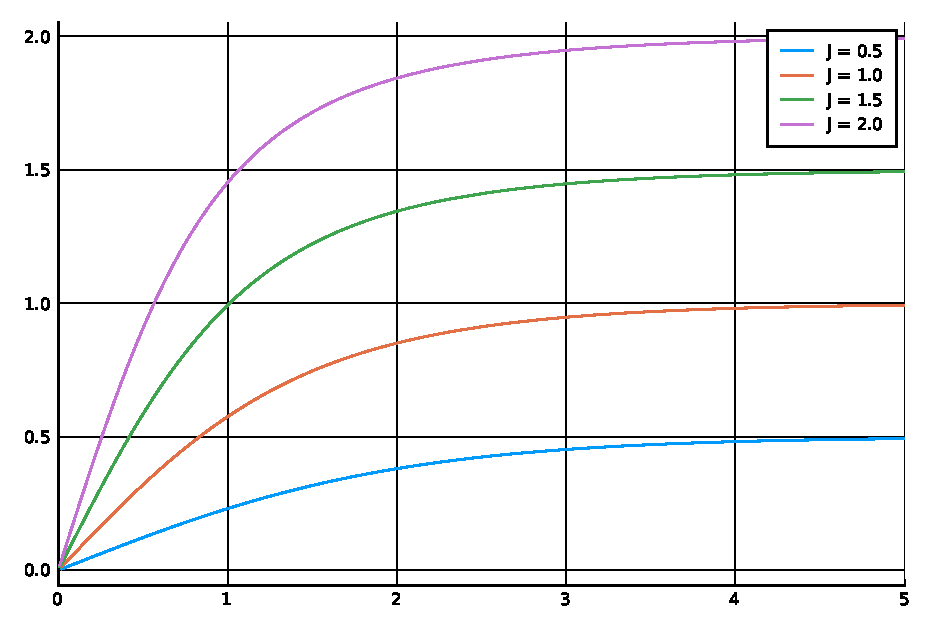
\includegraphics[width=0.6\textwidth]{img/brillouin.eps}
    \caption{График $M^z(\alpha)$. В отрицательную сторону симметрично.}
    %\label{fig:}
\end{figure}
В слабых полях 
\begin{equation*}
	M^z = N g_J \mu_\text{Б} \frac{J(J+1)}{3} \frac{g_J \mu_\text{Б} H}{T} = N \frac{(g_J \mu_\text{Б})^2}{3 T}J (J+1) H.
\end{equation*}
\begin{itemize}
	\item  $g_J m_B H \ll T$ -- слабое поля ($\alpha \ll 0$): $\chi = N \frac{(g_J\mu_\text{Б})^2}{3 T}J (J+1) \sim \frac{1}{T}$ -- закон Кюри;
	\item $g_J m_B H \gg T$ -- сильное поле ($\alpha \gg 0$): $M^{z} = g_J \mu_\text{Б} N J$.
\end{itemize}

\subsection*{Каноническое распределение для классического газа}
Теперь $N$ атомов как-то двигаются в объёме $V$, и задана температура $T$. Реализации такого макросостояния можно добиться по-разному.
\begin{equation*}
	Z = \sum e^{- H(\smallvc{p}_i, \smallvc{r}_i)/T} = \int d \Gamma e^{- H(\smallvc{p}_i, \smallvc{r}_i)/T} 
\end{equation*}
Плотность состояний
\begin{equation*}
	d \Gamma =  \frac{1}{N!}\left(\frac{1}{(2 \pi \hbar)^3}\right)^N d^3 p_1 d^3 r_1 d^3 p_2 d^3 r_2 \ldots d^3 p_N d^3 r_N
	=
	\frac{1}{N!} \frac{\prod_{i = 1}^N d^3 p_i d^3 r_i}{(2 \pi \hbar)^{3N}}.
\end{equation*}
То есть придётся взять интеграл
\begin{equation*}
	Z = \int \frac{1}{N!} \frac{\prod_{i = 1}^N d^3 p_i d^3 r_i}{(2 \pi \hbar)^{3N}} e^{- H(\smallvc{p}_i, \smallvc{r}_i)/T}.
\end{equation*}

\section{Cеминар}
\subsection*{Термодинамические  функции классического больцмановского газа}
Продолжаем, то что было с прошлого раза.
\begin{equation*}
	p = (\vc{p}_1, \vc{p}_2, \ldots, \vc{p}_N),
	\hspace{1 cm}
	r = (\vc{r}_1, \vc{r}_2, \ldots, \vc{r}_N).
\end{equation*}
Предположим только, что частицы не взаимодействуют, и не в поле тяжести, тогда
\begin{equation*}
	Z = \int \frac{1}{N!} \frac{d^3 p_1 }{(2 \pi \hbar)^{3}} \ldots \frac{d^3 p_N }{(2 \pi \hbar)^{3}} \underbrace{\int d^3 r_1 \ldots d^3 r_N}_{V} e^{-\frac{p_1^2 + \ldots + p_N^2}{2 m T}}=
	\frac{V^N}{N!} \left(\int \frac{d^3 p}{(2 \pi \hbar)^3} e^{- \frac{p^2}{2 m T}}\right)^N
\end{equation*}
Получили интеграл, который отражает по смыслу квантовый объём $J = 1/V_Q$:
\begin{equation*}
	J = \int \frac{d^3}{(2 \pi \hbar)^3} e^{- \frac{p^2}{2 m T}} = \frac{(2 \pi m T)^{2/3}}{(2 \pi \hbar)^{3}},
	\hspace{1 cm}
	V_Q = \frac{(2 \pi \hbar)^3}{(2 \pi m T)^{2/3}} = \left(\frac{h}{\sqrt{2 \pi m T}}\right)^{3}
\end{equation*}
То есть статвес будет
\begin{equation*}
	Z = \frac{V^N}{N!} J^N = \frac{V^N}{N!} \frac{1}{V_Q^N},
\end{equation*}
Теперь введём тепловой импульс
\begin{equation*}
	p_T = \sqrt{2 \pi m T}
	\hspace{1 cm}
	\Rightarrow
	\hspace{1 cm}
	\lambda_T = \frac{h}{p_T} = \frac{h}{\sqrt{2 m E}},
\end{equation*}
где $\lambda_T$ -- тепловая длина волна де-Бройля, через неё сразу удобно выразить квантовый объём
\begin{equation*}
	V_Q = (\lambda_T)^3 = \left(\frac{2 \pi \hbar^2}{MT}\right)^{3/2}
\end{equation*}
Физический смысл $V_Q$
\begin{itemize}
	\item газ рассматриваем как классический, когда $\frac{V}{N} \gg V_q$;
	\item газ рассматриваем как квантовый, когда $\frac{V}{N} < V_Q$.
\end{itemize}
То есть при какой-то температуре -- температуре вырождения -- мы начинаем считать газ квантовым.
\begin{equation*}
	T = T_\text{выр}:
	\hspace{1 cm}
	\frac{V}{N} \simeq V_Q
	\hspace{0.5 cm}
	\Rightarrow
	\hspace{0.5 cm}
	\frac{1}{n} \simeq \left(\frac{2 \pi \hbar^2}{m T_\text{выр}}\right)^{2/3}.
\end{equation*}
Таким образом
\begin{equation*}
	T_\text{выр} \sim \frac{\hbar^2}{m} n^{2/3}.
\end{equation*}
\begin{itemize}
	\item  для атомов: $m \sim 10^{-23}$ г, $n \sim 10 ^{19}$ см$^3$ будет $T_\text{выр} \sim 0.1 $ К;
	\item для электронов $m \sim 10^{-27}$ г, $n \sim 10 ^{22}$ см$^3$ будет $T_\text{выр} \sim 10^4-10^5 $ К
\end{itemize}

Продолжим работу со статсуммой, возьмём формулу Стирлинга
\begin{equation*}
	Z = \frac{V^N}{N!} \frac{1}{V_Q^N}, = \left(\frac{e V}{N}\right)^{N} \frac{1}{V_Q},
	\hspace{1 cm}
	N! \simeq \left(\frac{N}{e}\right)^{N}.
\end{equation*}
А свободная энергия для классического газа
\begin{equation*}
	F = - T \ln Z = - T N \ln \frac{e V}{N} \frac{1}{V_Q(T)}.
\end{equation*}
Ну а теперь зная свободную энергию можно навырожать ещё кучу всего
\begin{equation*}
	d F = - S d T - P d V + \mu d N.
\end{equation*}
\begin{equation*}
	\mu = \left(\frac{\partial F}{\partial N}\right)_{T, V} = - T \ln \frac{e V}{N} \frac{1}{V_Q} + T N \underbrace{\frac{\partial}{\partial N} \ln N \tilde{f}(V,T)}_{1/N} = - T \ln \frac{V}{N} \frac{1}{V_Q}.
\end{equation*}
Так получаем химический потенциал больцмановского газа
\begin{equation*}
	\mu(T, V, N) = - T \ln \frac{V}{N} \left(\frac{m T}{2 \pi \hbar^2}\right)^{3/2}.
\end{equation*}
\begin{figure}[h]
    \centering
    \includegraphics[width=0.5\textwidth]{img/sem5im1.pdf}
    %\caption{}
    %\label{fig:}
\end{figure}

Можно подумать что значит отрицательный химический потенциал
\begin{itemize}
	\item  $\Delta F = \mu \Delta N$ --- при добавлении частицы в систему свободная энергия уменьшается;
	\item $\mu = (\partial E/\partial N)_{S,V}$, а $E = \frac{3}{2} N T (S,V, N)$ --- при добавлении частицы при постоянной температуре энергия возрастет, надо быть аккуратным.
\end{itemize}
Ещё смысл -- число частиц в квантовом объёме в классическом газе должно быть мало, поэтому $\mu < 0$ из следующих соображений:
\begin{equation*}
	e^{\mu/T} = n V_Q \ll 1.
\end{equation*}

Теперь можно получить давление
\begin{equation*}
	P(T, V, N) = \left(-\frac{\partial F}{\partial V}\right)_{T, N} = T N \frac{\partial}{\partial V} \ln V \tilde{\tilde{f}}(N,T)
	\hspace{1 cm}
	\Rightarrow
	\hspace{1 cm}
	P = \frac{N}{V} T.
\end{equation*}

 И получим ещё энтропию
 \begin{equation*}
 	S = \left(- \frac{\partial F}{\partial T}\right)_{V, N} = N \ln \frac{e V}{N} \frac{1}{V_Q} + \underbrace{T N \frac{\partial}{\partial T} \ln T^{3/2} \tilde{\tilde{\tilde{f}}}}_{\frac{3}{2}N}
 	= N \ln\frac{V}{N}\frac{1}{V_Q} + N + \frac{3}{2} N.
 \end{equation*}
 Получили так называемую формулу Сакура-Тетроде -- получаем ту самую константу, с точностью до которой мы её не знали из термодинамики!
 \begin{equation*}
 	S = N \left[\ln \frac{V}{N}\frac{1}{V_Q} + \frac{5}{2}\right].
 \end{equation*}

 Теперь повыражаем энергию
 \begin{equation*}
 	E = F + TS = F + T \left(- \frac{\partial F}{\partial T}\right) = - T \ln Z + T \frac{\partial }{\partial T} T \ln Z = - T \ln Z + T \ln Z + T^2 \frac{\partial}{\partial T} \ln Z,
 \end{equation*}
 то есть
 \begin{equation*}
 	E(T, V, N) = T^2 \frac{\partial}{\partial T} \ln Z.
 \end{equation*}
А $Z$ мы знаем (для классического газа сейчас работаем везде)
\begin{equation*}
	E = T^2 N \frac{\partial}{\partial T} \ln T^{3/2} \tilde{\tilde{\tilde{\tilde{f}}}}(V, N) = T^{2} N \frac{3}{2} \frac{1}{T} = \frac{3}{2} N T
	\hspace{1 cm}
	\Rightarrow
	\hspace{1 cm}
	E = \frac{3}{2} N T.
\end{equation*}
На этом кажется с классическим газом у нас всё.
Решим теперь задачу
\subsection*{Вращательная теплоёмкость}
Ну понятно, что молекула может двигаться не только поступательно, но и вращательно. Рассмотрим двухатомную молекулу. У неё есть энергия связанная с вращением
\begin{equation*}
	E_\text{вращ} = \frac{\vc{L}^2}{2 I},
	\hspace{1 cm}
	I = M R_0^2,
\end{equation*}
где $M$ -- приведенная масса, $R_0$ -- расстояние между молекулами.
Передём к гамильтониану такого движения
\begin{equation*}
	\hat{H}_\text{вращ} = \frac{\hbar^2}{2 I} \hat{\vc{L}}^2
	\hspace{1 cm}
	\Rightarrow
	\hspace{1 cm}
	E_L = \frac{\hbar^2}{2 I} L(L+1).
\end{equation*}
Получили уровни энергию вырожденную $g = 2L +1$ раз, тогда статсумма
\begin{equation*}
	Z_{1\text{ вращ}} = \sum_{L=0}^{\infty} (2 L +1) e^{- E_L/T} = 
	\sum_{L=0}^{\infty} (2 L +1) e^{- \frac{\hbar^2}{2 I} \frac{L (L+1)}{T}}
\end{equation*}
Масштаб энергий кванта вращательной энергии $T_C = \frac{\hbar^2}{2 I} \sim 1 - 10$ К.

Будем работать в приближении \textbf{классического рассмотрения} --- $T \gg T_c$, то есть экспонента в статсумме меняется плавно, слабо, пока $L \leq L_max$, которое определяется $\frac{T_c}{T} L_{max}^2 \approx 1$.
Ну то есть до $L_{max}$ -- сумму заменяю интегралом, а далее всё экспоненциально подавлено 
\begin{equation*}
	Z_{1 \text{ вращ}} = \int_{0}^{+\infty} (2L+1) e^{- \frac{T_c}{T}L (L+1)} d L = \frac{T}{T_c}.
\end{equation*}
Отсюда
\begin{equation*}
	E_{1 \text{ вращ}} = T^2 \frac{\partial}{\partial T} \ln Z_{1 \text{вращ}} = T^2 \frac{\partial}{\partial T} \ln \frac{T}{T_c} = T
	\hspace{1 cm}
	\Rightarrow
	\hspace{1 cm}
	\frac{C_\text{вращ}}{N} = c_{1 \text{вращ}} = 1.
\end{equation*}
И вот казалось бы всё хорошо, теплоёмкость двухатомного газа $5/2$, класс. Но если мы начнём его охлаждать, то заметим, что она в какой-то момент резко падает до $3/2$.

Поэтому нужно поработать в \textbf{квантовом режиме} --- $T \leqslant T_c$. Тут уже и сумму на интеграл не заменить, и вообще грустно, зато компьютер сравнительно такое небольшое число частиц посчитает быстро.
\begin{equation*}
	Z_{1\text{ вращ}}  = 
	\sum_{L=0}^{\infty} (2 L +1) e^{- \frac{T_c}{T} \frac{L (L+1)}{T}}
\end{equation*}
Тут ещё придется задуматься о том, например, для молекулы из одинаковых атомов со спинами, например $s_{1,2} = 1/2$ (для $H_2$). И вот тут заиграет ферми и бозе статистики, ведь от суммарного спина $S = 0, 1$ будет выцепляться симметричность 
\begin{itemize}
	\item параводород $S= 0$, тогда $L = 0, 2, 4, 6, \ldots$;
	\item ортоводород $S= 1$, тогда $L = 1, 3, 5, 7, \ldots$;
\end{itemize}
То есть
\begin{equation*}
	Z_{1 \text{ вращ}}^\text{пара} = \sum_{L = 0, 2, 4 \ldots} = 1 + s e^{- 6 \frac{T_c}{T}} + \ldots
\end{equation*}
\begin{equation*}
	E_{1 \text{ вращ}}^\text{пара} = T^2 \frac{\partial}{\partial T} \ln\left(1 + s e^{- 6 \frac{T_c}{T}} + \ldots \right) = 30 T_c e^{-6 T_c/T} + \ldots
\end{equation*}
\begin{equation*}
	C_{1 \text{ вращ}}^\text{пара} = \frac{d E}{d T} = \frac{180 T_c^2}{T^2} e ^{- 6 T_c/T} + \ldots
\end{equation*}
Для орто водорода теперь
\begin{equation*}
	Z_{1 \text{ вращ}}^\text{орто} = 3 e^{- 2 T_c/T} + 7 e^{-12 T_c/T} + \ldots
\end{equation*}



\section{Cеминар}
\subsection*{продолжаем}
\begin{equation*}
	Z_{1 \text{ вращ}}^\text{орто} = \sum_{L = 1,2,5 \ldots} =3 e^{- 2 T_c/T} + 7 e^{-12 T_c/T} + \ldots
\end{equation*}
Энергия вращаетльного движения тогда
\begin{equation*}
	E_{1 \text{ вращ}}^\text{орто} = T^2 \frac{\partial}{\partial T} \ln Z_{1 \text{ вращ}}^\text{орто} = T^2 \frac{\partial}{\partial T} \ln 3 e^{- 2 T_c /T}\left(1 + \frac{7}{3} e^{-10 T_c/T} + \ldots \right)
	= T^2 \frac{\partial}{\partial T} \left(- \frac{2 T_c}{T} + \frac{7}{3} e^{-10 \frac{T_c}{T}}\right) = 2 T_c + \frac{70}{3} e^{- 10 T_c/T}.
\end{equation*}
И тогда
\begin{equation*}
	C_{1 \text{ вращ}}^\text{орто} = \frac{700}{3} \frac{T_c^2}{T^2} e^{-10 T_c/T} + \ldots.
\end{equation*}
\red{нарисовать график}

Может показаться, что к единице ничего не стремится, но
\begin{equation*}
	Z_{1 \text{ вращ}}^\text{орто} = \int_{0}^{+\infty} d L (2 L + 1) e^{-L(L+1)T_c/T} = \frac{T}{T_c}
	\hspace{0.5 cm}
	\leadsto
	\hspace{0.5 cm}
	E_{1 \text{ вращ}}^\text{орто} = T^2 \frac{\partial}{\partial T} \ln \frac{T}{T_c} = T
	\hspace{0.5 cm}
	\leadsto
	\hspace{0.5 cm}
	C_{1 \text{ вращ}}^\text{орто} = 1.
\end{equation*}
Теперь в качестве упражнения можно рассмотреть смесь в состоянии термодинамического равновесия орто + пара водород $N_\text{орто} + N_\text{пара} = N$. Показать, что
\begin{equation*}
	\frac{N_\text{орто}(T)}{N_\text{пара}(T)} = 3 \frac{Z_\text{орто}(T)}{Z_\text{пара}(T)}.
\end{equation*}
Перейдём к теории флуктуаций\footnote{Сейчас у меня сядет ноут, потому что в 520ГК не работает розетка. Поэтому возможно когда-то (когда ещё и первый семинар) появится и эта часть конспекта.}
\subsection*{Термодинамические квазиравновесные флуктуации}
\subsubsection*{Изолированное тело}
Рассматриваем изолированное тело, хотим посмотреть вероятность находится в неравновесном состоянии, задаваемом параметром $x$ -- отклонение от равновесного состояния. 
\begin{equation*}
	w(x) \sim \frac{\text{число всех микростостояний отвечающих } x}{\text{полное число всех возможных микросостояний}} \sim \text{статвес состояния } x \sim e^{S(x)}.
\end{equation*}
\begin{equation*}
	S(x) = S(x_0) + \Delta S,
	\hspace{1 cm}
	\Rightarrow
	\hspace{1 cm}
	w(x) \sim e^{\Delta S(x)}
\end{equation*}
где $S(x_0)$ -- отвечает равновесию системы.

\subsubsection*{Тело в среде}
Среда есть термостат. К телу относятся переменные $\{S,V,T,P\}$, а к термостату относятся $\{S_0, V_0, T_0, P_0\}$ -- и он всегда в равновесии.
Вводим снова параметр $x$ -- харакатеризующий отклонение состояние тела от равновесия
\begin{equation*}
	w(x) \sim e^{\Delta S_\text{tot}(x)},
	\hspace{1 cm}
	\Delta S_\text{tot} = \Delta S + \Delta S_0.
\end{equation*}
Мы считаем, что состояние тремостата остаётся равновесным. ТО есть $T_0$ и $P_0$ остаются постоянными.
Тогда для него справедлив второй закон термодинамики
\begin{equation*}
	\Delta S_0 = \frac{\delta Q_0}{T_0} = - \frac{\delta Q}{T_0}.
\end{equation*}
Ну а тепло ему, кроме как от тела получат неоткуда.

А вот тело, хоть и отклоняется от равновесия, но всегда можем записать первый закон
\begin{equation*}
	\delta Q = \Delta E + A_\text{против сил внешнего давления} = \Delta E + P_0 \Delta V,
\end{equation*}
так как внешнее давление это и есть $P_0$.
Таким образом получаем для энтропии теромтстата
\begin{equation*}
	\Delta S_0 = - \frac{\Delta E + P_0  \Delta V}{T_0}
	\hspace{1 cm}
	\Rightarrow
	\hspace{1 cm}
	\Delta S_\text{tot} = \Delta S - \frac{\Delta E + P_0 \Delta V}{T_0} = \frac{T_0 \Delta S - \Delta E - P_0  \Delta V}{T_0}.
\end{equation*}
Таким образом 
\begin{equation*}
	w(x) \sim \exp\left(\frac{T_0 \Delta S - \Delta E - P_0  \Delta V}{T_0}\right),
	\hspace{1 cm}
	x = \{\Delta S, \Delta V, \Delta E\}.
\end{equation*}

Теперь предположим, что флуктуации малы. Тогда $E(S,V)$ имеет тот же функциональный вид, тот же самый, как и в равновесии.


\section{Cеминар}
\subsection*{Флуктуации числа частиц в газе}
Возьмем $N$ частиц газа в объёме $V$. Зададимся вопросом какова вероятность найти в небольшом объёме газа $v$ ровно $n$ частиц? То есть $P_n(v) - ?$. Введём вероятность $p = v/V$ одной частицы попасть в объём в $v$. Соответственно $q = 1 - v/V$ --- это вероятность того, что частицы не находятся в этом объёме.

Тогда для $n$ частиц получим вероятность просто по биномиальному распределению
\begin{equation*}
	P_n(v) = C_N^n p^n q^{N-n}. 
\end{equation*}
Проследим как оно плавно перетекает в распределение Пуассона. Вообще биномиальный коэффициент --- достаточно сложная штука, но мы будем работать в приближении, что $v \ll V$ ($p\ll 1$), и будет нам счастье. В этом случае введём параметр $\lambda = N p$. Его физический смысл \begin{equation*}
	\lambda = N \frac{v}{V} = \frac{N}{V}v = n_\text{концентрация} \cdot v = \text{среднее число частиц в }  v = \overline{n}.
\end{equation*}
Понятно, что для параметра $\lambda$ возможны разные случаи: $\lambda < 1$, $\lambda \sim 1$ и $\lambda >1$.

Зафиксируем $\lambda$, тогда вероятности находиться и не находиться в объёме $v$
\begin{equation*}
	p^n = \left(\frac{\lambda}{N}\right)^n,
	\hspace{1 cm}
	q^{N-n} = \left(1 - \frac{\lambda}{N}\right)^{N-n}.
\end{equation*}
Вероятность тогда
\begin{equation*}
	P_n(v) = \frac{N (N-1)\ldots(N-n+1)}{n!} \frac{\lambda^n}{N^n} \frac{\left(1 - \frac{n}{N}\right)^N}{1 - \left(\frac{\lambda}{N}\right)^n}
	= \frac{\lambda^n}{n!} \frac{N(N-1) \ldots (N-n+1)}{N \cdot N \ldots N} \frac{\left(1 - \frac{\lambda}{N}\right)}{\left(1 - \frac{\lambda}{N}\right)N}.
\end{equation*}
Теперь, $n$ у нас --- фиксировано,а $N \gg 1$, тогда
\begin{equation*}
	\frac{N(N-1) \ldots (N-n+1)}{N \cdot N \ldots N} = 1 \left(1 - \frac{1}{N}\right)\ldots\left(1 - \frac{n-1}{N}\right) \longrightarrow 1, 
	\hspace{1 cm}
	N \to \infty,
\end{equation*}
\begin{equation*}
	\left(1 - \frac{\lambda}{N}\right)^n \longrightarrow 1,
	\hspace{1 cm}
	\left(1 - \frac{\lambda}{N}\right)^N \longrightarrow \exp(-\lambda).
\end{equation*}
В результате получили, что биномиальное распределение перетекло в распределение Пуассона
\begin{equation*}
	P_n(v) \longrightarrow P(n,\lambda) = \frac{\lambda^n}{n!} \exp(-\lambda).
\end{equation*}
Его характеристика 
\begin{equation*}
	\langle n\rangle = \sum_{n=0}^{\infty} n P(n,\lambda) = \lambda,
	\hspace{1 cm}
	\langle \Delta n^2\rangle = \overline{n^2} - (\overline{n})^2 = \lambda.
\end{equation*}
Откуда получаем относительную флуктуацию
\begin{equation*}
	\frac{\sqrt{\langle \Delta n^2\rangle}}{\overline{n}} = \frac{1}{\sqrt{\overline{n}}} = \frac{1}{\sqrt{\lambda}} \longrightarrow 0,
	\hspace{1 cm}
	\overline{n} \gg 1
	\hspace{2 mm}
	(\lambda \gg 1).
\end{equation*}
И можно заметить, что, при таких малых относительных флуктуациях,  распределение Пуассона переходит в распределение Гаусса
\begin{equation*}
	\varphi_{\overline{n}, \sigma} = \frac{1}{\sqrt{2 \pi \sigma^2}} \exp\left\{-\frac{(n -\overline{n})^2}{2 \sigma^2}\right\},
	\hspace{1 cm}
	\sigma^2 =\lambda.
\end{equation*}
\begin{figure}[h]
    \centering
    \includegraphics[width=0.5\textwidth]{img/sem7im1.pdf}
    %\caption{}
    %\label{fig:}
\end{figure}
Пик находится в $n = \overline{n} = \lambda$. Формально
\begin{equation*}
	P(n, \lambda) \longrightarrow \frac{1}{\sqrt{2 \pi \lambda}} \exp\left\{-\frac{(n-\lambda)^2}{2 \lambda}\right\}.
\end{equation*}
Как это делается? Сначала раскладываем в ряд $P(n,\lambda) = e^{w(n)}$ около $n = \lambda$
\begin{equation*}
	w(n) = w(\lambda) + \frac{1}{2}w''(\lambda) (n-\lambda)^2 + \ldots
\end{equation*}
У нас же $P(n,\lambda) = \frac{\lambda^n}{n!}e^{-\lambda}$, то есть
\begin{equation*}
	w(n) = \ln\left\{ - \lambda\frac{\lambda^n}{n!}\right\}
	=
	n \ln \lambda - \lambda - \ln n! = n \ln \lambda - \lambda n \ln n + n - \frac{1}{2} \ln 2\pi n,
\end{equation*}
где мы воспользовались формулой Стирлинга
\begin{equation*}
	n! \approx \left(\frac{n}{e}\right)^n \sqrt{2 \pi n},
	\hspace{1 cm}
	\Rightarrow
	\hspace{1 cm}
	\ln n! \approx n \ln n - n + \frac{1}{2} \ln 2 \pi n.
\end{equation*}
И так возможно, внимательный читатель задался вопросом, почему в разложении нет первой производной 
\begin{equation*}
	w'(n) = \ln \lambda -  \ln n - 1 + 1 - \underbrace{\frac{1}{2 n}}_\text{крайне мала},
	\hspace{1 cm}
	w'(n) = 0
	\hspace{0.5 cm}
	\Rightarrow
	\hspace{0.5 cm}
	n = \lambda.
\end{equation*}
Как видно, пик вообще узкий, поэтому там, где распределение вообще отлично от нуля, у нас везде максимум и первой производной мы пренебрегаем.
Вторая же производная будет
\begin{equation*}
	w''(n) = - \frac{1}{n}\mid_{n=\lambda} = -\frac{1}{\lambda}.
\end{equation*}
Итого получаем разложение
\begin{equation*}
	w(n) = \ln \frac{1}{\sqrt{2 \pi \lambda}} + \frac{1}{2 \lambda} (n - \lambda)^2.
\end{equation*}
Тогда 
\begin{equation*}
	e^{w(n)} = \frac{1}{\sqrt{2 \pi \lambda}} \exp \left\{-\frac{(n-\lambda)^2}{2 \lambda}\right\} = P(n,\lambda)
\end{equation*}
Получился Гаусс! Забавно, что даже при таком допущении у нас и нормировка тоже сошлась. А всё почему?
\begin{flushright}
 	 Потому что пик очень узкий. 
 \end{flushright}

\subsection*{Неравновесная энтропия}
Будем работать на примере Ферми статистики. Пусть есть уровень энергии системы $ \varepsilon$ вырожденный $g$ раз. И на этом уровне есть $n$ частиц ($0<n<g$).

Число всех микросостояний системы $=$ число способов разместить $n$ частиц по $g$ ячейкам.
\begin{equation*}
	W = C_g^n = \frac{g!}{n! (g - n)!}.
\end{equation*}

Теперь усложняем. Пусть будет $j$ уровней с энергией $\varepsilon_i$, каждый из них вырожден $g_i$ раз и на каждом $n_i$ частиц ($i = 1,\ldots,j$).
При этом число частиц на уровнях меняется, но так, чтобы сохранилось только суммарное число частиц и суммарная энергия системы
\begin{equation*}
	\sum_i n_i = N,
	\hspace{1 cm}
	\sum_i \varepsilon_i n_i = E.
\end{equation*}
Таким образом фиксируем $N, E$, что является весьма жестким ограничением для системы.

Ищем же мы $E(n_1, n_2, \ldots, n_j, \ldots) = E(\{n_j\})$.
А именно, хотим найти кратность вырождения с заданным фиксированным набором ${n_j}$ энергии $E \equiv$ статвесу макросостояния $(N,E)$. $W(N,E) - ?$
\begin{equation*}
	W = \prod_{j} W_j,
\end{equation*}
где $j$ -- нижний индекс по (??).
$\{n_j\}$ -- не просто любой набор,но ещё и удовлетворяющий закону сохранению числа частиц и энергии.

Пусть мы нашли кратность вырождения уровня с $E$, так что все ${n_j}$ -- фиксированные, и \textbf{неравновесная энтропия}
\begin{equation*}
	S = \ln W(N, E, {n_j}).
\end{equation*}
Здесь нужно, подчеркнуть, что $S(\{n_j\})$ -- энтропия именно от набора, который доставляет ей максимум. 
И тогда, если $S(N,E, \{n_j\})$ $\Rightarrow$ $S$ будет равновесной термодинамической энтропией $S(E,N)$ (набор фиксированный).

Все наши рассуждения упирались в то, что набор $\{n_j\}$ должен быть достаточно удачный, найдём же такой набор, что доставит максимум энтропии. Если посмотреть выше, то видно, что всё уже у нас для поиска этого набора есть
\begin{equation*}
	S = \sum_j = \big[\ln g_j ! - \ln n_j ! - \ln(g_j - n_j)!\big]
		=
		\sum_j \big[g_j \ln g_j - n_j \ln n_j - (g_j - n_j) \ln(g_j - n_j)\big]
\end{equation*}
И не забываем, что выполнятся должны
\begin{equation*}
	\sum_j n_j = N,
	\hspace{0.5 cm}
	\hspace{0.5 cm}
	\sum_j \varepsilon_j n_j = E.
\end{equation*}
Чтобы найти такие $n_j$ которые доставляют энтропии максимум и учесть условия, воспользуемся формулой Лагранжа
\begin{equation*}
	\tilde{S} = S + \alpha N + \beta E
	\hspace{1 cm}
	\leadsto
	\hspace{1 cm}
	\frac{\partial \tilde{S}}{\partial{n_j}} = 0.
\end{equation*}
По отдельности
\begin{equation*}
	\frac{\partial S}{\partial n_j} = - \ln n_j - 1 + \ln(g_j - n_j) + 1 = - \ln \frac{n_j}{g_j	- n_j},
	\hspace{1 cm}
	\frac{\partial N}{\partial n_j} = 1,
	\hspace{1 cm}
	\frac{\partial E}{\partial n_j} = \varepsilon_j.
\end{equation*}
Таким образом получаем
\begin{equation*}
	- \ln \frac{n_j}{g_j - n_j} + \alpha + \beta \varepsilon_j = 0
	\hspace{1 cm}
	\Rightarrow
	\hspace{1 cm}
	\frac{n_j}{g_j - n_j} = e^{\alpha + \beta \varepsilon_j} = \chi,
\end{equation*}
далее
\begin{equation*}
	n_j = g_j \chi - n_j \chi 
	\hspace{0.5 cm}
	\Rightarrow
	\hspace{0.5 cm}
	(1 + \chi) n_j = g_j \chi
	\hspace{0.5 cm}
	\Rightarrow
	\hspace{0.5 cm}
	n_j = g_j \frac{\chi}{1 + \chi} = g_j \frac{e^{\alpha + \beta \varepsilon_j}}{1 + e^{\alpha + \beta \varepsilon_j}}.
\end{equation*}
Вот именно такие числа $n_j$ заполнения доставляют максимум энтропии.
Для окончательной радости нам остаётся только найти $\alpha$ и $\beta$.

Сравним полученную формулу Лагранжа с известным нам дифференциалом
\begin{equation*}
	d S + \alpha d N + \beta d E = 0
	\hspace{1 cm}
	\longleftrightarrow
	\hspace{1 cm}
	d S + \frac{\mu}{T} d N - \frac{1}{T} d E - \frac{P}{T} d V = 0.
\end{equation*}
Раз мы в задаче фиксируем уровни $\varepsilon_j$, то они, являясь функцией $V$ (частицы в ящике) фиксируют и объём: $V = \const$ $\Rightarrow$ $d V = 0$.

Тогда не трудно сравнить оставшиеся члены и понять, что
\begin{equation*}
	\alpha = \frac{\mu}{T},
	\hspace{1.5 cm}
	\beta = - \frac{1}{T}.
\end{equation*}
Для $S$ термодинамической энтропии хоть вынь хоть положь, эти частицы. И ей же и является доставленная в максимум статистическая энтропия $d S + \alpha d N + \beta d E$.

Подставляя коэффициента $\alpha, \beta$ получаем что 
\begin{equation*}
	n_i = g_i \frac{1}{e^{\frac{\varepsilon_i - \mu}{T}}+1}
	\hspace{1 cm}
	\leadsto
	\hspace{1 cm}
	\frac{n_i}{g_i} = f_i = \frac{1}{e^{\frac{\varepsilon_i - \mu}{T}}+1},
\end{equation*}
где $f_i$ -- числа заполнения $i$-го уровня. А вся эта красота называется распределением Ферми-Дирака.

А теперь остаётся просуммировать по всем наборам.
Среди этих сумм одно слагаемое сильно перевешивает все остальные. Оно и будет давать главный вклад в энтропию, прямо как в начале семинара, где мы рассуждали про острый пик.